%%%%%%%%%%%%%%%%%%%%%%%%%%%%%%%%%%%%%%%%%
% Beamer Presentation
% LaTeX Template
% Version 1.0 (10/11/12)
%
% This template has been downloaded from:
% http://www.LaTeXTemplates.com
%
% License:
% CC BY-NC-SA 3.0 (http://creativecommons.org/licenses/by-nc-sa/3.0/)
%
%%%%%%%%%%%%%%%%%%%%%%%%%%%%%%%%%%%%%%%%%

%----------------------------------------------------------------------------------------
%	PACKAGES AND THEMES
%----------------------------------------------------------------------------------------

\documentclass{beamer}

\mode<presentation> {

\usetheme{AnnArbor}
}

\usepackage{graphicx} % Allows including images
\usepackage{booktabs} 
\usepackage[utf8]{inputenc}
\usepackage{multirow}

\graphicspath{{Pictures/}} 

\title{Statističko testiranje očekivanja}
\author{Neven \textsc{Miculinić}}

\institute[FER] % Your institution as it will appear on the bottom of every slide, may be shorthand to save space
{
Fakultet Elektrotehnike i Računarstva \\ % Your institution for the title page
\medskip
\textit{neven.miculinic@fer.hr} % Your email address
}
\date{}

\begin{document}

\frame{\titlepage}

\begin{frame}
	\frametitle{Uvod u Statističko testiranje}
	\begin{itemize}[<+->]
		\item Postupak donošenja odluke o odbacivanju ili ne odbacivanju statističke hipoteze zove se testiranje statističkih hipoteza 
		\item Provodi kada se mora donijeti neka odluka (ono je binarno)
	\end{itemize}
\end{frame}

\begin{frame}
	\frametitle{Uzorak i Statistika}
	\begin{itemize}[<+->]
		\item Uzorak $n$-torka $(x_1, \ldots, x_n)$
		\item Statistika $f($ $X_1 , X_2 , \ldots X_n$ $)$
	\end{itemize}
\end{frame}

\begin{frame}
	\frametitle{Statističke Hipoteza}
	\begin{itemize}[<+->]
		\item Statistička hipoteza je (bilo koja) pretpostavka o
		(populacijskoj) razdiobi od X 
		\item Nul hipoteza $H_0$
		\item Altrenativna hipoteza $H_a$
	\end{itemize}
\end{frame}

\begin{frame}
	\frametitle{Primjeri Hipoteza}
	\begin{itemize}[<+->]
		\item na FERu je 99\% muškaraca
		\item dnevno 1000 studenata FFZG idu u Cassandru
		\item Varijanca bodova na SISu je 15
	\end{itemize}
\end{frame}

\begin{frame}
	\frametitle{Primjeri Hipoteza}
	\begin{figure}
		\centering
		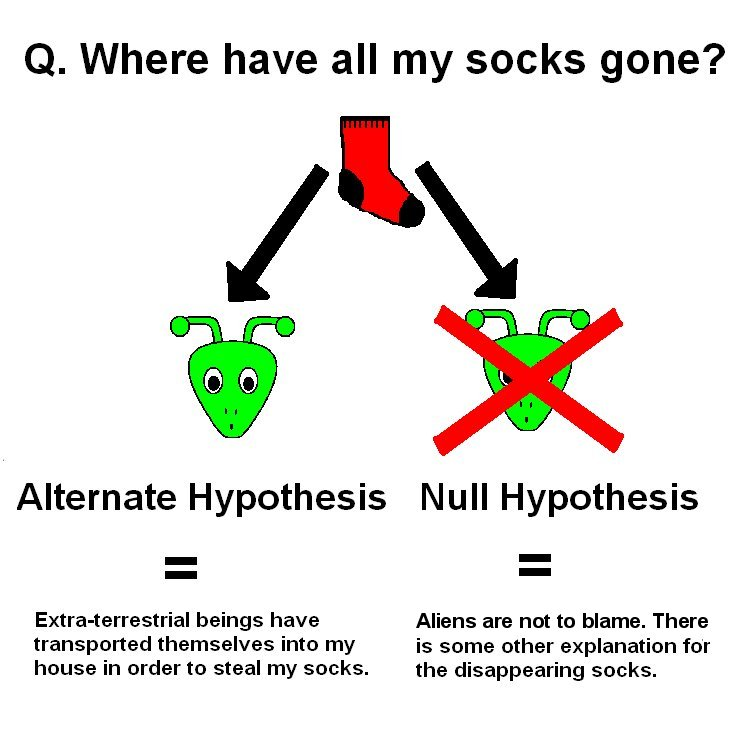
\includegraphics[width=\textwidth,height=0.8\textheight,keepaspectratio]{aliens.jpg}
	\end{figure}
\end{frame}

\begin{frame}
	\frametitle{Greške}
	\begin{figure}
		\centering
		\begin{table}[h]
			\resizebox{\textwidth}{!}{%
			\begin{tabular}{cc|c|c|}
			\cline{3-4}
			 &  & \multicolumn{2}{c|}{Nul hipoteza je} \\ \cline{3-4} 
			 &  & Točna & Netočna \\ \hline
			\multicolumn{1}{|c|}{\multirow{2}{*}{Presuda testa je:}} & Odbaci & \begin{tabular}[c]{@{}c@{}}Greška 1. vrste\\ Lažno pozitivni\\ $P = \alpha$\end{tabular} & Točno \\ \cline{2-4} 
			\multicolumn{1}{|c|}{} & Prihvati & Točno & \begin{tabular}[c]{@{}c@{}}Greška 2. vrste\\ Lažno negativni \\ $P = \beta$\end{tabular} \\ \hline
			\end{tabular}
			}
		\end{table}	
	\end{figure}
\end{frame}

\begin{frame}
	\frametitle{Područje prihvaćanja}

	\begin{block}{Nivo značajnosti testa}
		$\alpha$ - definira se kao vjerojatnost u slučaju istinitosti $H_0$ test odbaci $H_0$
	\end{block} \pause

	\begin{block}{Snaga testa}
		$1-\beta$ - definira se kao vjerojatnost odbacivanja $H_0$ u slucaju njene neistinitosti
	\end{block} \pause

	\begin{block}{Područje prihvaćanja}
		Konstruira se interval nad kojem se statistika uzorka prihvaća s značajnošću $\alpha$
	\end{block}
\end{frame}

\begin{frame}
	\frametitle{}
	\begin{figure}
		\centering
		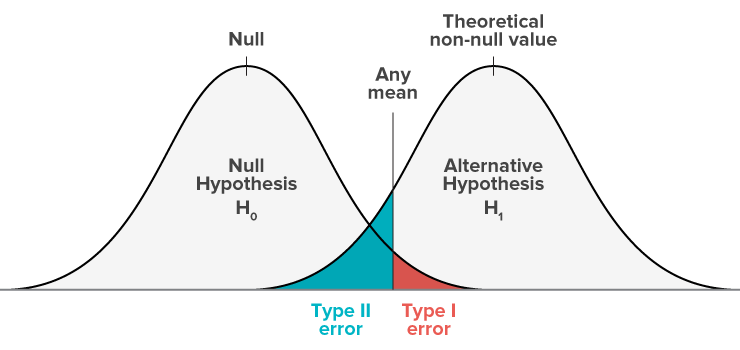
\includegraphics[width=\textwidth,height=0.8\textheight,keepaspectratio]{type12.png}
	\end{figure}
\end{frame}


\begin{frame}
	\frametitle{P vrijednosti}
	p vrijednost se definira kao najmanja značajnost test, $\alpha$, za koju bi ovaj uzorak presudili odbacivanjem nul hipoteze, $H_0$

	\begin{figure}[ph]
	    \centering
	    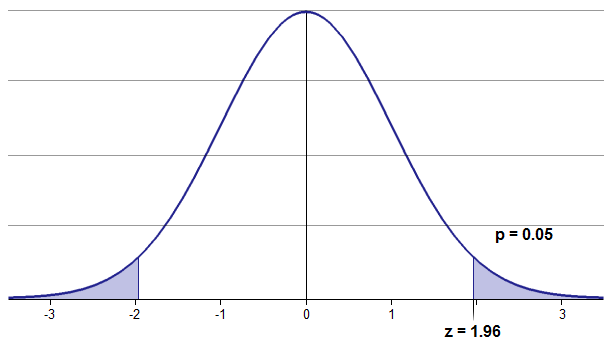
\includegraphics[width=0.9\textwidth,height=0.7\textheight,keepaspectratio]{pvalue2.png}
	    \caption{P vrijednost statistike $\mu = 0$ s distribucijom $X \sim \mathcal{N}(0,1)$}
		\label{fig:pvalue2}
	\end{figure}
\end{frame}

\begin{frame}
	\frametitle{$t$ distribucija}
	\begin{figure}
		\centering
	    \includegraphics[width=0.9\textwidth,height=0.7\textheight,keepaspectratio]{Student_t.jpg}
	\end{figure}
\end{frame}

\begin{frame}
	\frametitle{Statističko testiranje očekivanja}
	\begin{block}{Pretpostavke}
		\begin{itemize}
			\item Populacija je normalno distribuirana
			\item uzorci su medusobno nezavisni
		\end{itemize}
	\end{block}
	\pause
	\begin{block}{Hipoteza}
		\begin{itemize}
			\item $H_0:\; \bar{x} = \mu$
			\item $H_a:\; \bar{x} \ne \mu$
		\end{itemize}
	\end{block}
	\pause
	\begin{block}{Statistika}
		\[\frac{\sqrt{n} (\bar{x} - \mu)}{s} \sim t_{n-1}\]
	\end{block}
	\pause
	\begin{block}{Područje prihvaćanja}
		\[
		\bar{x} \in \left<\mu - \frac{s}{\sqrt{n}} \cdot t_{n-1, \frac{\alpha}{2}}, \mu + \frac{s}{\sqrt{n}} \cdot t_{n-1, \frac{\alpha}{2}} \right> \]

	\end{block}
\end{frame}

\begin{frame}
	\frametitle{Zaključak}
	\begin{figure}
		\centering
		\huge Zaključak
	\end{figure}

	\begin{itemize}[<+->]
		\item Često nam je nul hipoteza suprotna od onoga što želi dokazati
		\item Ovakvi jednostavniji testovi bitni su za dokazivanje pretpostavka koje rabe snažniji testovi
		\item t-test jedan od načešćih testova 
	\end{itemize}
\end{frame}

\begin{frame}
	\Huge{\centerline{Pitanja?}}
\end{frame}

\end{document} 